\chapter{Analyse}
    Hier ein neues Kapitel
    Viele Zitate: \autocite[]{patterson} \autocite[]{krizhevsky} \autocite[]{matlab} \cite{pitts} \cite{lawrence} \cite{miesbach}
    \section{Anforderungen}
        Eine Section
        \subsection{Echtzeitfähigkeit}
            \begin{figure}[h]
                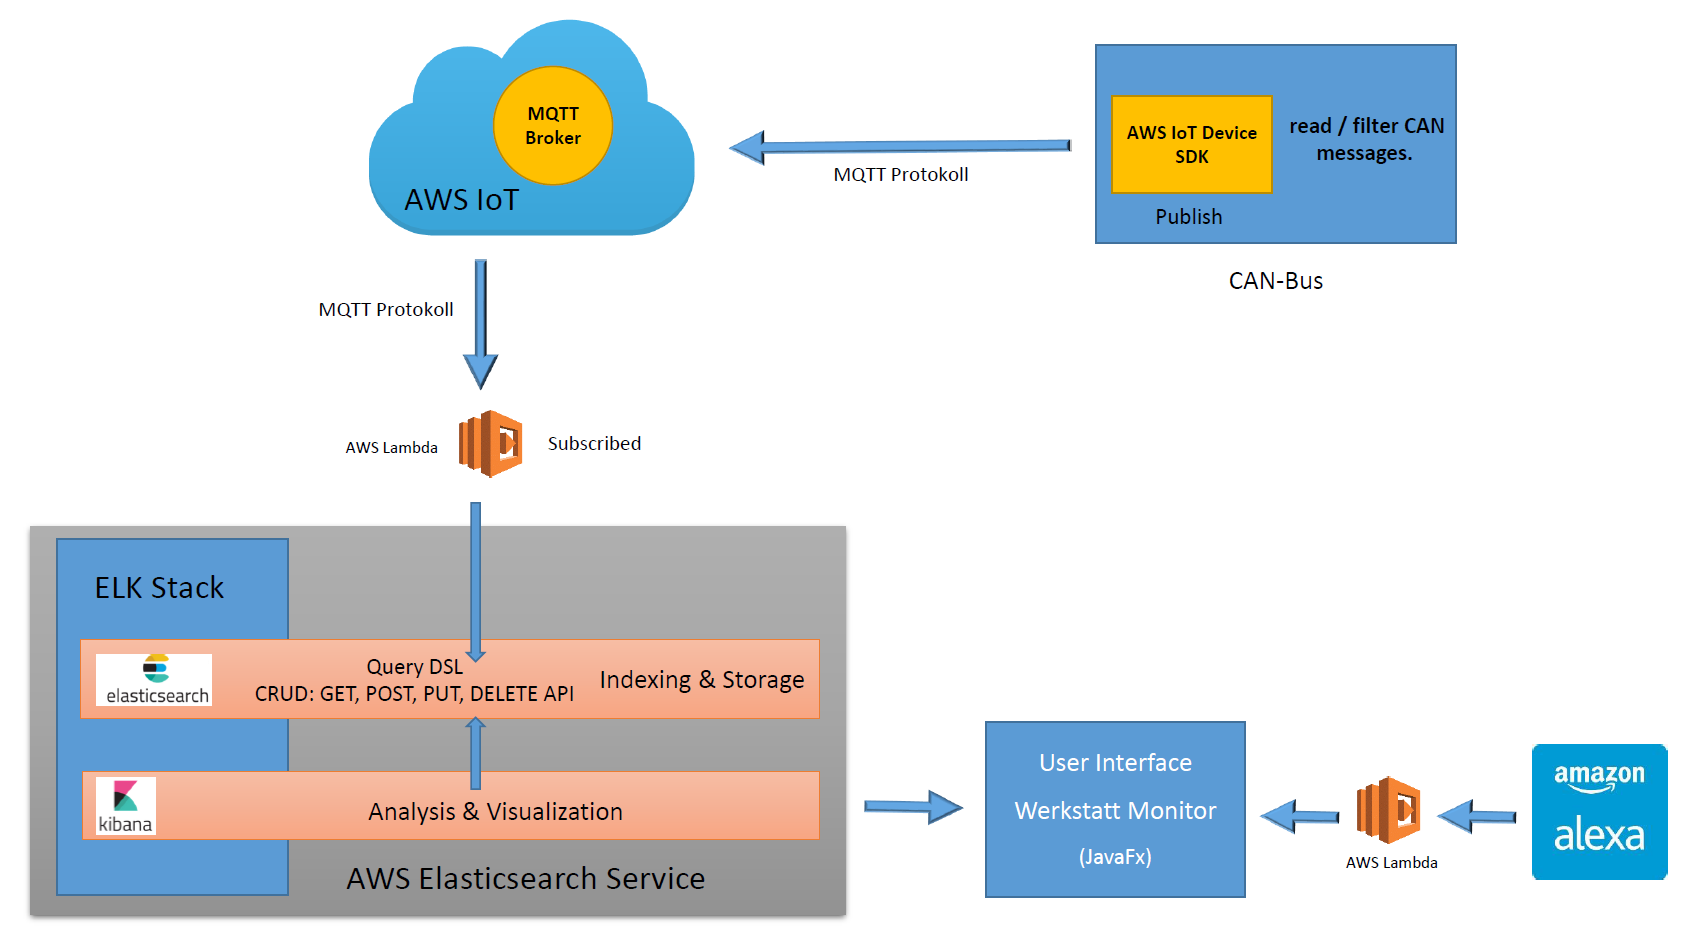
\includegraphics[scale=0.2]{Abbildungen/Kapitel3/Big-architecture.png}
                \centering
                \caption{das Architekturbild}
                \label{Abb:Architekturbild}   
            \end{figure}  
             \begin{table}[h]
                \begin{tabular}{ccc}
                      \hline
                      Spalte1 & Spalte2 & Spalte3\\                      
                      \hline
                      1 & 2 & 3\\
                      \hline
                \end{tabular}
                \centering
                \caption{Variation über Zeit}
                \label{Tab:Tabelle3}
            \end{table}
            
Hier eine neue Tabelle   
            
            \begin{table}[h]
                \begin{tabular}{ccc}
                      \hline
                      Spalte1 & Spalte2 & Spalte3\\                      
                      \hline
                      1 & 2 & 3\\
                      \hline
                \end{tabular}
                \centering
                \caption{new added Tabelle}
                \label{Tab:New added}
            \end{table}
 
        
        
    \section{dynamische Erstellung von Diagramme}
        Eine Subsection
        \newpage
        Eine neue Seite
        \newpage 
        Noch eine neue Seite
        \newpage    
        und noch eine neue Seite